% ---------------------------------------------------------------------------------------------------------------
% TEMPLATE PARA TRABALHO DE CONCLUSÃO DE CURSO
% Universidade Tecnológica Federal do Paraná - UTFPR
% Customização da classe abnTeX2 (http://www.abntex.net.br/) para as normas da UTFPR
%
% Autores: Diego Marczal
% 	       Michael Vornes <https://github.com/mvornes>
% Adaptação (DACOM-CP): Silvio Ricardo Rodrigues Sanches
%
%----------------------------------------------------------------------------------------------------------------
% Codificação: UTF-8
% LaTeX:  abnTeX2          
% ---------------------------------------------------------------------------------------------------------------


% CARREGA CLASSE PERSONALIZADA DA UTFPR--------------------------------------------------------------------------
\documentclass[%twoside,                   % Impressão em frente e verso
    	        oneside,                   % Impressão apenas frente
]{configuracoes/utfpr-abntex2}


% INCLUI ARQUIVOS DE CONFIGURAÇÕES-------------------------------------------------------------------------------
% REFERÊNCIAS------------------------------------------------------------------
\usepackage[%
    alf,
    abnt-emphasize=bf,
    bibjustif,
    recuo=0cm,
    abnt-url-package=url,       % Utiliza o pacote url
    abnt-refinfo=yes,           % Utiliza o estilo bibliográfico abnt-refinfo
    abnt-etal-cite=3,
    abnt-etal-list=3,
    abnt-thesis-year=final
]{abntex2cite}                  % Configura as citações bibliográficas conforme a norma ABNT

% PACOTES----------------------------------------------------------------------
\usepackage[utf8]{inputenc}                                 % Codificação do documento
\usepackage[T1]{fontenc}                                    % Seleção de código de fonte
\usepackage{booktabs}                                       % Réguas horizontais em tabelas
\usepackage{color, colortbl}                                % Controle das cores
\usepackage{float}                                          % Necessário para tabelas/figuras em ambiente multi-colunas
\usepackage{graphicx}                                       % Inclusão de gráficos e figuras
\usepackage{icomma}                                         % Uso de vírgulas em expressões matemáticas
\usepackage{indentfirst}                                    % Indenta o primeiro parágrafo de cada seção
\usepackage{microtype}                                      % Melhora a justificação do documento
\usepackage{multirow, array}                                % Permite tabelas com múltiplas linhas e colunas
\usepackage{subeqnarray}                                    % Permite subnumeração de equações
\usepackage{lastpage}                                       % Para encontrar última página do documento
\usepackage{verbatim}                                       % Permite apresentar texto tal como escrito no documento, ainda que sejam comandos Latex
\usepackage{amsfonts, amssymb, amsmath}                     % Fontes e símbolos matemáticos
\usepackage[algoruled, portuguese]{algorithm2e}             % Permite escrever algoritmos em português
%\usepackage[scaled]{helvet}                                % Usa a fonte Helvetica
\usepackage{times}                                          % Usa a fonte Times
%\usepackage{palatino}                                      % Usa a fonte Palatino
%\usepackage{lmodern}                                       % Usa a fonte Latin Modern
\usepackage[bottom]{footmisc}                               % Mantém as notas de rodapé sempre na mesma posição
\usepackage{ae, aecompl}                                    % Fontes de alta qualidade
\usepackage{latexsym}                                       % Símbolos matemáticos
\usepackage{lscape}                                         % Permite páginas em modo "paisagem"
%\usepackage{picinpar}                                      % Dispor imagens em parágrafos
%\usepackage{scalefnt}                                      % Permite redimensionar tamanho da fonte
%\usepackage{subfig}                                        % Posicionamento de figuras
%\usepackage{upgreek}                                       % Fonte letras gregas

% Redefine a fonte para uma fonte similar a Arial (fonte Helvetica)
\renewcommand*\familydefault{\sfdefault}

% CONFIGURAÇÕES DE APARÊNCIA DO PDF FINAL--------------------------------------
\makeatletter
\hypersetup{%
    portuguese,
    colorlinks=true,   % true: "links" coloridos; false: "links" em caixas de texto
    linkcolor=blue,    % Define cor dos "links" internos
    citecolor=blue,    % Define cor dos "links" para as referências bibliográficas
    filecolor=blue,    % Define cor dos "links" para arquivos
    urlcolor=blue,     % Define a cor dos "hiperlinks"
    breaklinks=true,
    pdftitle={\@title},
    pdfauthor={\@author},
    pdfkeywords={abnt, latex, abntex, abntex2}
}
\makeatother

% ALTERA O ASPECTO DA COR AZUL--------------------------------------------------
\definecolor{blue}{RGB}{41,5,195}

% REDEFINIÇÃO DE LABELS---------------------------------------------------------
\renewcommand{\algorithmautorefname}{Algoritmo}
\def\equationautorefname~#1\null{Equa\c c\~ao~(#1)\null}

% CRIA ÍNDICE REMISSIVO---------------------------------------------------------
\makeindex

% HIFENIZAÇÃO DE PALAVRAS QUE NÃO ESTÃO NO DICIONÁRIO---------------------------
\hyphenation{%
    qua-dros-cha-ve
    Kat-sa-gge-los
}



% INCLUI ARQUIVOS DO TRABALHO DE CONCLUSÃO DE CURSO (PRÉ-TEXTUAIS, TEXTUAIS, PÓS-TEXTUAIS)-----------------------

% INSERE CAPA E FOLHA DE ROSTO
% CAPA---------------------------------------------------------------------------------------------------

% ORIENTAÇÕES GERAIS-------------------------------------------------------------------------------------
% Caso algum dos campos não se aplique ao seu trabalho, como por exemplo,
% se não houve coorientador, apenas deixe vazio.
% Exemplos: 
% \coorientador{}
% \departamento{}

% DADOS DO TRABALHO--------------------------------------------------------------------------------------
\titulo{Introduzindo boas práticas em engenharia de software utilizando a plataforma arduino}
\titleabstract{Title in English}
\autor{Guilherme Gonçalves Borges da Silva}
\autorcitacao{Silva, Guilherme} % Sobrenome em maiúsculo
\local{Cornélio Procópio}
\data{2018}

% NATUREZA DO TRABALHO-----------------------------------------------------------------------------------
% Opções: 
% - Trabalho de Conclusão de Curso (se for Graduação)
% - Dissertação (se for Mestrado)
% - Tese (se for Doutorado)
% - Projeto de Qualificação (se for Mestrado ou Doutorado)
\projeto{Trabalho de Conclusão de Curso}

% TÍTULO ACADÊMICO---------------------------------------------------------------------------------------
% Opções:
% - Bacharel ou Tecnólogo (Se a natureza for Trabalho de Conclusão de Curso)
% - Mestre (Se a natureza for Dissertação)
% - Doutor (Se a natureza for Tese)
% - Mestre ou Doutor (Se a natureza for Projeto de Qualificação)
\tituloAcademico{Engenharia de Computação}

% ÁREA DE CONCENTRAÇÃO E LINHA DE PESQUISA---------------------------------------------------------------
% Se a natureza for Trabalho de Conclusão de Curso, deixe ambos os campos vazios
% Se for programa de Pós-graduação, indique a área de concentração e a linha de pesquisa
\areaconcentracao{}
\linhapesquisa{}

% DADOS DA INSTITUIÇÃO-----------------------------------------------------------------------------------
% Se a natureza for Trabalho de Conclusão de Curso, coloque o nome do curso de graduação em "programa"
% Formato para o logo da Instituição: \logoinstituicao{<escala>}{<caminho/nome do arquivo>}
\instituicao{Universidade Tecnológica Federal do Paraná}
\departamento{Departamento Acadêmico de Computação}
\programa{Curso de Engenharia de Computação}
\logoinstituicao{0.2}{dados/figuras/logo-instituicao.png} 

% DADOS DOS ORIENTADORES---------------------------------------------------------------------------------
\orientador{André Takeshi Endo}
%\orientador[Orientadora:]{Nome da orientadora}
\instOrientador{Universidade Tecnológica Federal do Paraná}

\coorientador{Paulo Augusto Nardi}
%\coorientador[Coorientadora:]{Nome da coorientadora}
\instCoorientador{Universidade Tecnológica Federal do Paraná}

% FOLHA DE ROSTO--------------------------------------------------------------------------------------------------------

% TRABALHO DE CONCLUSÃO DE CURSO
 \preambulo{{\imprimirprojeto} apresentado ao {\imprimirprograma} da {\imprimirinstituicao}, como requisito parcial para a obtenção do título de {\imprimirtituloAcademico}.}

% DISSERTAÇÃO DE MESTRADO
% \preambulo{{\imprimirprojeto} apresentada ao Programa de \mbox{Pós-graduação} da {\imprimirinstituicao}, como requisito parcial para obtenção do título de {\imprimirtituloAcademico}.}

% TESE DE DOUTORADO
% \preambulo{{\imprimirprojeto} apresentada ao Programa de \mbox{Pós-graduação} da {\imprimirinstituicao}, como requisito parcial para a obtenção do título de {\imprimirtituloAcademico}.}

% PROJETO DE QUALIFICAÇÃO DE MESTRADO OU DOUTORADO
%\preambulo{{\imprimirprojeto} apresentado ao Programa de \mbox{Pós-graduação} da {\imprimirinstituicao}, como requisito parcial para a obtenção do título de {\imprimirtituloAcademico}.}

% OBSERVAÇÕES-----------------------------------------------------------------------------------------------------------
% Altere este arquivo APENAS comentando as linhas que não se aplicam ao tipo de trabalho acadêmico desejado.


\begin{document}

\pretextual
\imprimircapa                                               	           % Comando para imprimir Capa
\imprimirfolhaderosto{}                                     		   % Comando para imprimir Folha de rosto
% INSERE ELEMENTOS PRÉ-TEXTUAIS
% DEDICATÓRIA------------------------------------------------------------------

\renewcommand{\dedicatorianame}{DEDICATÓRIA}

\begin{dedicatoria}

Altere este texto inserindo a dedicatória do seu trabalho. 

\end{dedicatoria}
          			   % Dedicatória
% AGRADECIMENTOS---------------------------------------------------------------

\begin{agradecimentos}[AGRADECIMENTOS] 

Agradeço a Deus pelo dom da vida.

Aos meus pais e todos familiares, que me apoiaram nos momentos difíceis e deram todo o suporte para que eu chegasse até aqui.

Ao meu professor orientador Prof. Dr. André Takeshi Endo, pela dedicação, ensinamentos e apoio na elaboração deste trabalho.

A todos os professores e funcionários desta Universidade, que contribuíram para minha formação.

Agradeço também aos amigos que fiz nesta Universidade, em especial, Caio Vinicius, Guilherme Farah, Matheus Giacomini e Raphael Ochetski.

E a todos que diretamente ou indiretamente fizeram parte da minha formação, o meu muito obrigado.

\end{agradecimentos}
        			   % Agradecimentos
% EPÍGRAFE---------------------------------------------------------------------

\renewcommand{\epigraphname}{EPÍGRAFE}

\begin{epigrafe}

\textit{Eu denomino meu campo de Gestão do Conhecimento, mas você não pode gerenciar conhecimento. Ninguém pode. O que pode fazer - o que a empresa pode fazer - é gerenciar o ambiente que otimize o conhecimento. (PRUSAK, Laurence, 1997).}

\end{epigrafe}

% OBSERVAÇÕES------------------------------------------------------------------
% Altere o texto para inserir a epígrafe do seu trabalho
              			   % Epígrafe
% RESUMO--------------------------------------------------------------------------------

\begin{resumo}[RESUMO]
\begin{SingleSpacing}

% Não altere esta seção do texto--------------------------------------------------------
\imprimirautorcitacao. \imprimirtitulo. \imprimirdata. \pageref {LastPage} f. \imprimirprojeto\ – \imprimirprograma, \imprimirinstituicao. \imprimirlocal, \imprimirdata.\\
%---------------------------------------------------------------------------------------
\textit{Contexto:} A engenharia de \textit{software} é uma disciplina fundamental para cursos de tecnologia, com objetivo de prover organização, qualidade e produtividade no desenvolvimento de \textit{software}. A disciplina é ministrada predominantemente de maneira teórica, tornando as aulas tediosas e em muitos momentos desmotivantes. Para suprir este problema em cursos de Engenharia, este tema pode ser abordado de maneira diferente, tendo em vista o foco dessas áreas em circuitos e componentes eletrônicos. \textit{Objetivo:} Neste contexto, este trabalho visa a utilização da plataforma Arduino em conjunto com conceitos de gamificação, uma nova tendência para aumentar motivação, engajamento e desempenho, para apoiar o ensino de engenharia de \textit{software}. Em particular, será desenvolvida uma aplicação web utilizando conceitos de gamificação para apoiar o ensino de engenharia de \textit{software} e descrever os resultados obtidos em relação a sua utilização. \textit{Método:} A aplicação será composta por metas, regras, um sistema de \textit{feedback} e a utilização da mesma deverá ser de forma voluntária, caracterizando os quatro traços definidores de um jogo. Além disso, um questionário será aplicado para os alunos da disciplina, visando a obtenção dos resultados obtidos através da utilização da aplicação. 

\textbf{Palavras-chave}: Engenharia de Software. Arduino. Gamificação. Educação em Engenharia.

\end{SingleSpacing}
\end{resumo}

% OBSERVAÇÕES---------------------------------------------------------------------------
% Altere o texto inserindo o Resumo do seu trabalho.
% Escolha de 3 a 5 palavras ou termos que descrevam bem o seu trabalho 
             			   % Resumo em Português
% ABSTRACT--------------------------------------------------------------------------------

\begin{resumo}[ABSTRACT]
\begin{SingleSpacing}

% Não altere esta seção do texto--------------------------------------------------------
\imprimirautorcitacao. \imprimirtitleabstract. \imprimirdata. \pageref {LastPage} f. \imprimirprojeto\ – \imprimirprograma, \imprimirinstituicao. \imprimirlocal, \imprimirdata.\\
%---------------------------------------------------------------------------------------

Elemento obrigatório em tese, dissertação, monografia e TCC. É a versão do resumo em português para o idioma de divulgação internacional. Deve ser antecedido pela referência do estudo. Deve aparecer em folha distinta do resumo em língua portuguesa e seguido das palavras representativas do conteúdo do estudo, isto é, das palavras-chave. Sugere-se a elaboração do resumo (Abstract) e das palavras-chave (Keywords) em inglês; para resumos em outras línguas, que não o inglês, consultar o departamento / curso de origem.\\

\textbf{Keywords}: Word. Second Word. Another word.

\end{SingleSpacing}
\end{resumo}

% OBSERVAÇÕES---------------------------------------------------------------------------
% Altere o texto inserindo o Abstract do seu trabalho.
% Escolha de 3 a 5 palavras ou termos que descrevam bem o seu trabalho 
             		           % Resumo em Inglês
% Lista de Figuras----------------------------------------------------------------

\pdfbookmark[0]{\listfigurename}{lof}
\listoffigures*
\cleardoublepage

% OBSERVAÇÕES---------------------------------------------------------------------
% Este arquivo não precisa de ser alterado, pois a lista é gerada automaticamente.
   % Lista de Figuras
% LISTA DE QUADROS----------------------------------------------------------------

\renewcommand{\listofquadrosname}{LISTA DE QUADROS}

\pdfbookmark[0]{\listofquadrosname}{loq}
\listofquadros*
\cleardoublepage

% OBSERVAÇÕES---------------------------------------------------------------------
% Este arquivo não necessita de ser editado. A lista é gerada automaticamente.
   % Lista de Quadros
% LISTA DE TABELAS-------------------------------------------------------------

\pdfbookmark[0]{\listtablename}{lot}
\listoftables*
\cleardoublepage

% OBSERVAÇÕES-------------------------------------------------------------------
% Este arquivo não precisa ser alterado, pois a lista é gerada automaticamente.
         		   % Lista de Tabelas
% LISTA DE ABREVIATURAS E SIGLAS----------------------------------------------------------

\begin{siglas}
    \item[DIY] Do It Yourself
    \item[ES] Engenharia de \textit{Software}
    \item[UML] Unified Modeling Language
\end{siglas}

% OBSERVAÇÕES-----------------------------------------------------------------------------
% Altere a lista acima para definir os acrônimos e siglas utilizados neste trabalho
          		   % Lista de Abreviaturas e Siglas
% LISTA DE SÍMBOLOS------------------------------------------------------------

\begin{simbolos}
    \item[$ \Gamma $] Letra grega Gama
    \item[$ \lambda $] Comprimento de onda
    \item[$ \in $] Pertence
\end{simbolos}

% OBSERVAÇÕES-------------------------------------------------------------------
% Altere a lista acima para definir os símbolos utilizados no trabalho
        		   % Lista de Símbolos
% LISTA DE ALGORITMOS----------------------------------------------------------

\newcommand{\algoritmoname}{Algoritmo}
\renewcommand{\listalgorithmcfname}{LISTA DE ALGORITMOS}

\floatname{algocf}{\algoritmoname}
\newlistof{listofalgoritmos}{loa}{\listalgoritmoname}
\newlistentry{algocf}{loa}{0}

\counterwithout{algocf}{chapter}
\renewcommand{\cftalgocfname}{\algoritmoname\space}
\renewcommand*{\cftalgocfaftersnum}{\hfill--\hfill}

\pdfbookmark[0]{\listalgorithmcfname}{loa}
\listofalgorithms
\cleardoublepage

% OBSERVAÇÕES------------------------------------------------------------------
% Este arquivo não precisa ser alterado, pois a lista é gerada automaticamente.
   % Lista de Algoritmos
% SUMÁRIO----------------------------------------------------------------------

\renewcommand{\contentsname}{SUMÁRIO}

\pdfbookmark[0]{\contentsname}{toc}
\tableofcontents*
\cleardoublepage

% OBSERVAÇÕES-------------------------------------------------------------------
% Este arquivo não precisa ser alterado, pois o sumário é gerado automaticamente.
               			   % Sumário

\textual
% INSERE ELEMENTOS TEXTUAIS
% INTRODUÇÃO-------------------------------------------------------------------

\chapter{INTRODUÇÃO}
\label{chap:introducao}


\section{OBJETIVOS}
\label{secobjetivos}

Tendo em vista o interesse de alunos de Bacharelado em Engenharia, ligados à tecnologia da informação, como Engenharia de Computação, Engenharia Elétrica e Engeharia de Software, em manter o contato com circuitos eletrônicos e o entretenimento causado por jogos no ensino, intensificando os conceitos adquiridos na teoria de forma prática \cite{thiry2010}, este trabalho tem por finalidade utilizar a plataforma arduino como motivação para introduzir boas práticas em engenharia de software através de um jogo educativo.                		           % Introdução
% FUNDAMENTACAO TEORICA------------------------------------------------------------------

\chapter{FUNDAMENTAÇÃO TEÓRICA}
\label{chap:fundamentacao-teorica}Este capítulo tem por finalidade a apresentação dos aspéctos teóricos e trabalhos relacionados, sendo constituído pelas seguintes seções: Seção 

\section{PLATAFORMA ARDUINO}
\label{sec:arduino} O arduino é uma plataforma de prototipagem eletrônica open-source criada em 2005, que baseia-se em hardware e software flexíveis e de fácil uso, tornando-se acessível para novatos e profissionais. O arduino é capaz de sentir o estado do ambiente através de sensores e interagir com o mesmo por meio de motores e outros atuadores, isto pode ser feito enviando um conjunto de instruções para o microcontrolador através da linguagem de programação Arduino e a IDE Arduino. Por ser uma plataforma open-source, possui uma vasta quantia de contribuições da comunidade mundial, composta por estudantes, programadores, artistas e profissionais, o que gera uma grande quantidade de conhecimento acessível, útil para usuários novatos e experientes \cite{arduino2018}.

Professores e alunos o utilizam a plataforma para o desenvolvimento de instrumentos científicos de baixo custo, ou para introduzir a programação e robótica, além de ser utilizada também por amadores, principalmente pelas seguintes características: baixo custo, as placas são mais baratas em comparação com outros microcontroladores. Multiplataforma, a IDE utilizada para o desenvolvimento de um sketch(nome dado aos programas, uma unidade de código que é carregada e executada em uma placa), chamada de Arduino Software, ´pode ser utilizada em sistemas operacionais Windows, Linux e Mac Os, diferenciando-se dos demais, limitados ao sistema operacional Windows. Ambiente de programação fácil e transparente, o Arduino Software é de fácil utilização e adaptável o suficiente para que usuários avançados tirem um melhor proveito da plataforma. Software open source e flexível, o software Arduino é uma ferramenta open source, podendo ser modificada e aprimorada por usuários experientes. A linguagem pode ser expandida através de bibliotecas em C++, além disto, pode-se adicionar trechos de código da linguagem de programação AVR-C nos programas do Arduino. Hardware open source e flexível, os planos das placas Arduino são publicados sob uma licena Creative Commons, permitindo o aprimoramento e criação de novos módulos.\cite{arduino2018}

\section{TESTE DE SOFTWARE}
\label{sec:testeDeSoftware} A computação evoluiu muito nas últimas décadas, sendo utilizada em diversas áreas da atividade humana, demandando qualidade e produtividade, e a engenharia de software acompanhou esse progresso, estabelecendo técnicas, critérios, métodos e ferramentas para o desenvolvimento de programas. A engenharia de software pode ser definida como uma disciplina que aplica os princípios da engenharia para a produção de softwares de alta qualidade e baixo custo\cite{Pressman1997}. Apesar dos métodos e técnicas empregadas na produção de softwares, ainda podem ocorrer erros no produto, e com o intuito de minimizar a ocorrência destes, algumas atividades são introduzidas ao longo de todo o processo de desenvolvimento, sendo o teste de software a mais utilizada \cite{Maldonado1997}, constituindo-se em um dos elementos para oferecer evidencias da confiabilidade do software.

Os testes de softwares são compostos por quatro etapas: planejamento de testes, projeto de caso de testes, execução e avaliação dos resultados dos testes, que são executadas ao longo do desenvolvimento do software e efetivam-se em três diferentes fases de teste: de unidade, de integração e de sistema. Onde o primeiro, dedica-se na menor unidade do projeto, identificando erros de lógica e implementação em cada parte do programa. O teste de integração é realizado durante a integração da estrutura do programa, e tem como objetivo, a partir dos módulos testados no nível de unidade, construir a estrutura do programa, na forma determinada pelo projeto. O teste de sistema, é realizado após a integração do sistema, identificando erros de funções e características de desempenho que não estejam na especificação.\cite{Maldonado2004}

\begin{figure}[!htb]
    \centering
    \caption{Modelo das etapas do teste de software}
    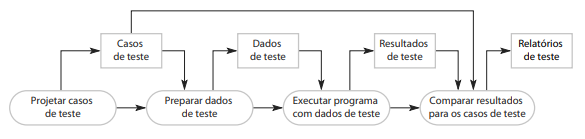
\includegraphics[width=1\textwidth]{./dados/figuras/Modelo_processo_de_software}
    \fonte{\cite{iansommerville}}
    \label{fig:figura-modelo-etapas-teste-de-software}
\end{figure}

As práticas pertinentes ao teste do software não abrangem somente a execução do programa, denominado teste dinâmico, existem também os testes estáticos, que não necessitam da execução de um software para serem realizados, podendo aplicá-los em diferentes artefatos como a revisão de documentos de requisitos e análise do código fonte.\cite{Pedro}

Os teste funcionais, conhecido como teste de caixa-preta e os testes estruturais, também chamados de teste de caixa-branca, são exemplos de técnicas de teste de software. No primeiro, não há a necessidade do testador conhecer a codificação, ele apenas informa os dados de entrada e examina se a saída está de acordo com o esperado, portanto os testes de caixa-preta visam detectar se o sistema aceita entradas incorretas, se a saída gerada está correta, se existem erros na interface e a falta de alguma funcionalidade. O segundo, observa a estrutura do código fonte para identificar a implementação e se os testes estão cobrindo diferentes caminhos, sendo assim, estes testes são implementados de forma a testar decisões logicas, variáveis estáticas, variáveis dinâmicas e \textit{loops}, por exemplo.\cite{Pedro}


\section{MANUTENÇÃO DE SOFTWARE}
\label{sec:manutencaoDeSoftware}

A vida de um sistema de computação não é finalizada após a sua implementação, ele ainda será utilizado por muito tempo, e com certeza passará por muitas atualizações, tanto para correção de erros ou apenas para otimização. Uma das fases do processo de desenvolvimento de software é a manutenção de software, este é um procedimento de melhoria de um programa que já foi desenvolvido, ou seja, já está em ambiente de produção, ou que ainda está em desenvolvimento. Com a manutenção também é realizado a correção dos erros encontrados por usuários do sistema ou testes realizados por desenvolvedores.

Existem diversas razões para que um software sofra alterações, principalmente se este implementar soluções aproximadas para problemas do mundo real, por exemplo, com o passar do tempo, conforme o melhor entendimento do problema, pode-se encontrar uma melhor solução, ou ainda, alterações de legislações de um determinado país ou novos requisitos do cliente.


\cite{rodrigoSpinola2011}

\section{PROCESSO DE SOFTWARE}
\label{sec:processoDeSoftware}      % Fundamentacao Teorica
\section{TRABALHOS RELACIONADOS}
\label{sec:trabalhos-relacionados}
\citeonline{utfpr2017} propõe em seu trabalho a produção de um recurso educacional para auxiliar o ensino de análise e projeto de \textit{software}. Para suprir a necessidade da prática em matérias de ES, principalmente para os cursos de Engenharia Elétrica, de Computação e Controle e Automação. O recurso educacional proposto consiste em um conjunto de projetos utilizando a plataforma Arduino. Cada projeto possui seis artefatos: o diagrama de casos de uso, o diagrama de atividades, o diagrama de maquinas de estado, o diagrama de classe, o esquemático de montagem e o código fonte em linguagem C/C++. A partir destes artefatos os alunos deveriam analisá-los e embarcá-los na plataforma Arduino, de forma a treinar a capacidade de interpretação de artefatos UML. Os artefatos foram aplicados em 3 turmas do curso de Engenharia de Computação da UTFPR - Câmpus Cornélio Procópio, durante a disciplina de Engenharia de \textit{Software}, onde após a conclusão da utilização, os alunos deram um \textit{feedback} através de um questionário baseado na escala \textit{likert} e uma questão aberta, para possíveis sugestões. As respostas a respeito do recurso educacional foram predominantemente positivas, demonstrando a aceitação pelos alunos e o auxílio no aprendizado.

\citeonline{Garcia2017} apresenta o GOAL (Gamification on Application Lifecycle Management), um \textit{framework} que tem como objetivo a orientação de um processo que suporta a introdução da gamificação em qualquer fase do desenvolvimento de \textit{software}. Um estudo de caso foi realizado pelos autores em uma empresa de desenvolvimento de \textit{software} para investigar a viabilidade de aplicação do \textit{framework} para integrar a gamificação em outros ambientes de engenharia de \textit{software}. Foram gamificadas três áreas de processo utilizando uma metodologia presente no GOAL, as áreas são: gerenciamento de requisitos, gerenciamento de projetos e teste de \textit{software}. Os elementos de jogos escolhidos para a gamificação foram: pontuação, \textit{levels}, distintivos, \textit{leaderboard}, \textit{social graph} e desafios. As conclusões obtidas em relação a utilização do \textit{framework} foram positivas, revelando benefícios oferecidos na utilização do GOAL em um contexto industrial. 

\chapter{PROPOSTA}
\label{chap:proposta}

Nesta seção são descritas as atividades que serão executadas a fim de atingir os objetivos deste trabalho, bem como as tecnologias utilizadas para o desenvolvimento do mesmo. Esta seção está subdivida em: plicação, ferramentas e utilização da aplicação e \textit{feedback} análise dos resultados.  

\section{APLICAÇÃO WEB}
\label{sec:desenvApp}



O artefato produzido por este trabalho será uma aplicação web, composta por uma breve introdução sobre a plataforma Arduino e um pequeno projeto a ser desenvolvido, para ambientar os usuários ao cenário. Após isso, será apresentado três áreas de conhecimentos abordadas no projeto, como apresentado na Figura \ref{fig:figura-areas-telas}, onde cada uma será constituída por uma introdução, questionário sobre conceitos e atividades práticas divididas em fases, como visto na Figura \ref{fig:figura-fases-telas}. O avanço em cada fase se dará somente após a resolução do exercício proposto e submissão para correção. A cada fase, o nível de complexidade do projeto será aumentado gradativamente.

\begin{figure}[!htb]
    \centering
    \caption{Áreas de conhecimento}
    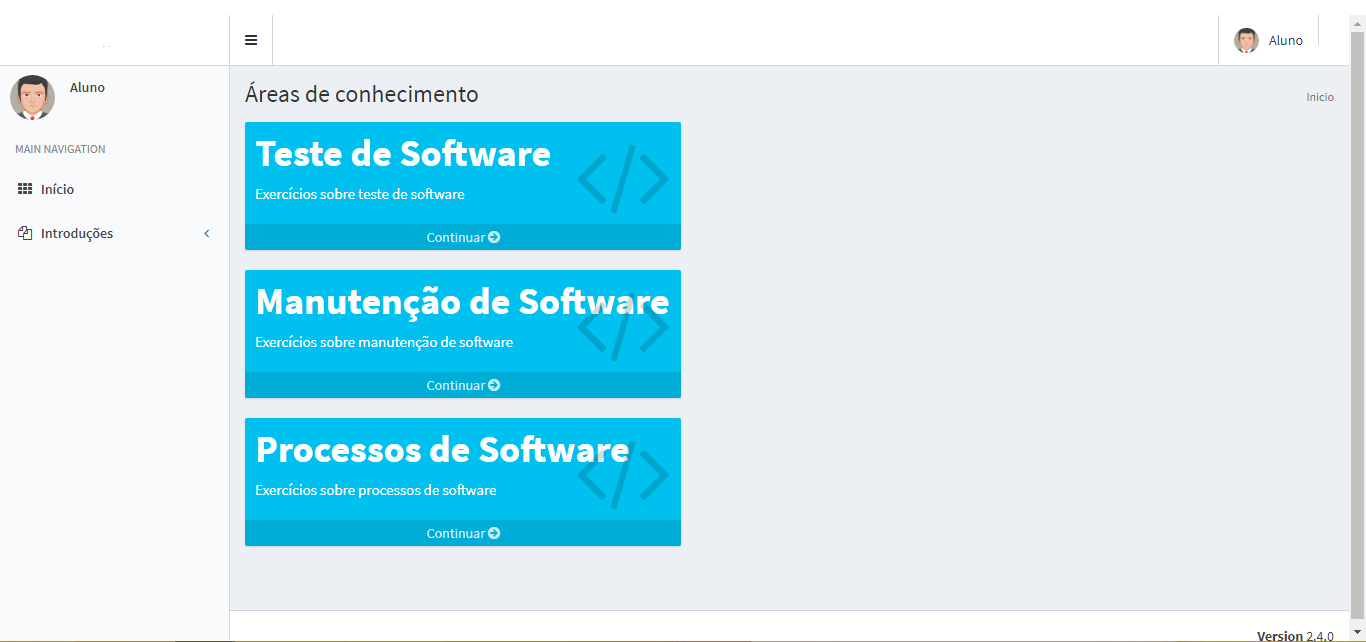
\includegraphics[width=1\textwidth]{./dados/figuras/areasTela}
    \fonte{Autoria Própria}
    \label{fig:figura-areas-telas}
\end{figure}

\begin{figure}[!htb]
    \centering
    \caption{Fases sobre teste de \textit{software}}
    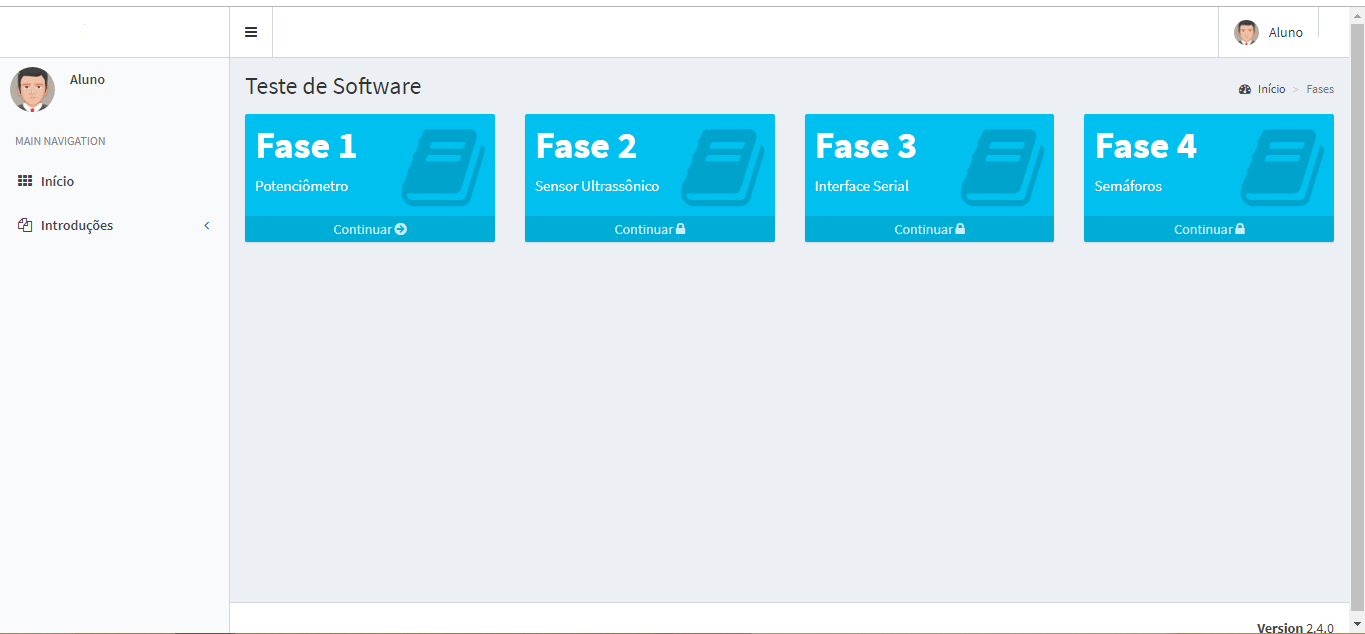
\includegraphics[width=1\textwidth]{./dados/figuras/fasesTela}
    \fonte{Autoria Própria}
    \label{fig:figura-fases-telas}
\end{figure}
 
Em cada fase será apresentado qual o objetivo, uma breve descrição, quais itens e componentes serão necessários, uma imagem do esquemático do projeto para montagem do circuito e um \textit{sketch}. Com essas informações o aluno deverá reconstruir o cenário proposto e realizar a atividade, que poderá surtir efeitos no \textit{sketch}, esquemático, diagramas de classe dos itens utilizados, diagramas de casos de uso, diagramas de atividade ou diagramas de máquina de estado do projeto. A Figura \ref{fig:figura-fase-tela} ilustra um exemplo de tela de uma das fases. Nela, o aluno realiza a leitura das atividades e tem acesso ao \textit{sketch}, esquemático e diagramas, para o auxílio na montagem do projeto. 
\begin{figure}[!htb]
    \centering
    \caption{Fase 1 - teste de \textit{software}}
    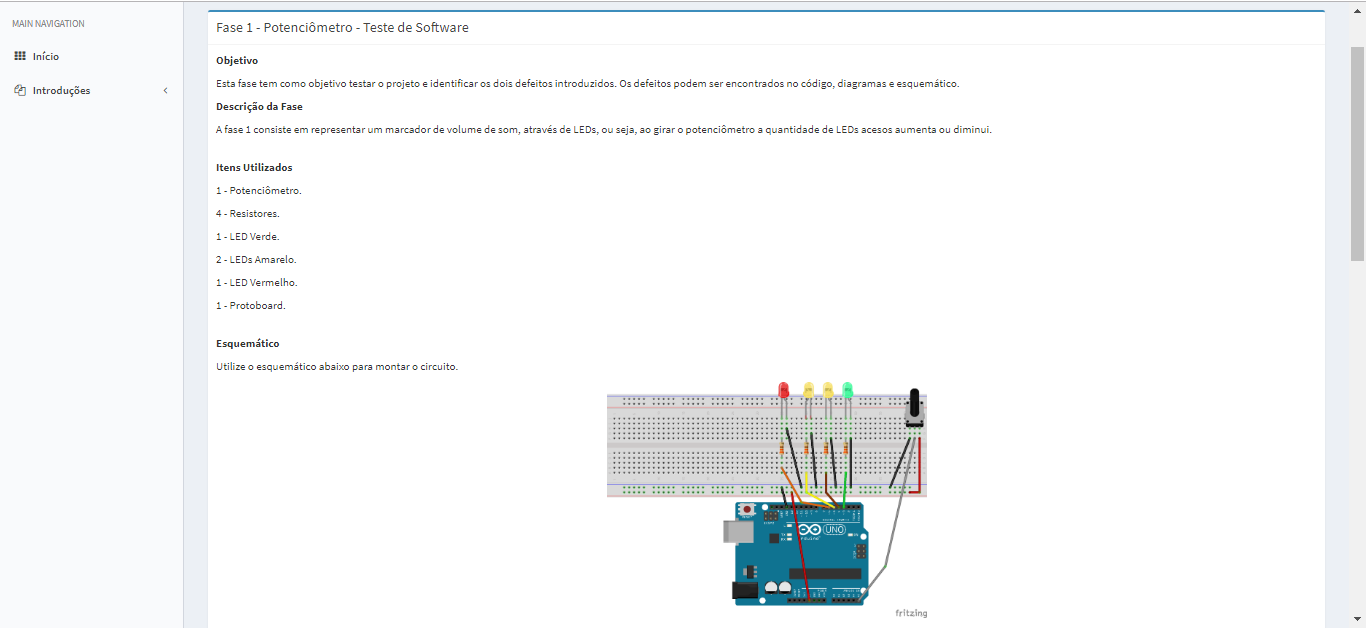
\includegraphics[width=1\textwidth]{./dados/figuras/faseTela}
    \fonte{Autoria Própria}
    \label{fig:figura-fase-tela}
\end{figure}

\section{FERRAMENTAS}
\label{sec:ferramentas}

\section{EXECUÇÃO DA APLICAÇÃO E ANÁLISE DE RESULTADOS}
\label{sec:execAppAnaliseResultados}
Para a avaliação da aceitação, motivação, engajamento, consolidação e aquisição de conhecimento causado pelo artefato gerado neste trabalho, o mesmo será utilizado por alunos da disciplina Engenharia de \textit{Software}, que possuem um conhecimento prévio sobre linguagem de programação, orientação a objetos, circuitos eletrônicos e alguns conceitos nos temas abordados neste trabalho. Ao término da utilização, os alunos darão um \textit{feedback} através de um questionário baseado na escala \texttt{likert}, um tipo de escala psicométrica comumente utilizada em pesquisas de opinião, onde a cada afirmação o pesquisado deve escolher um valor de 1 a 5. O valor um retrata o total desacordo ou negação, e o valor cinco representa o total acordo ou aceitação.


\chapter{CRONOGRAMA}
\label{chap:cronograma}                   % trabalhos-relacionados
% RESULTADOS-------------------------------------------------------------------

\chapter{ANÁLISE E DISCUSSÃO DOS RESULTADOS}

Cada capítulo deve conter uma pequena introdução (tipicamente, um ou dois parágrafos) que deve deixar claro o objetivo e o que será discutido no capítulo, bem como a organização do capítulo.
                    % Resultados
% ORIENTAÇÕES GERAIS------------------------------------------------------------


% SOBRE AS ILUSTRAÇÕES----------------------------------------------------------
\chapter{SOBRE AS ILUSTRAÇÕES}
\label{chap:apSobreIlust}

A seguir exemplifica-se como inserir ilustrações no corpo do trabalho. As ilustrações serão indexadas automaticamente em suas respectivas listas. A numeração sequencial de figuras, tabelas e equações também ocorre de modo automático.

Referências cruzadas são obtidas através dos comandos \verb|\label{}| e \verb|\ref{}|. Sendo assim, não é necessário por exemplo, saber que o número de certo capítulo é \ref{chap:fundamentacaoTeorica} para colocar o seu número no texto. Outra forma que pode ser utilizada é esta: \autoref{chap:fundamentacaoTeorica}, facilitando a inserção, remoção e manejo de elementos numerados no texto sem a necessidade de renumerar todos esses elementos.

% FIGURAS-----------------------------------------------------------------------
\chapter{FIGURAS}
\label{chap:figuras}

Exemplo de como inserir uma figura. A \autoref{fig:figura-exemplo1} aparece automaticamente na lista de figuras. Para saber mais sobre o uso de imagens no \LaTeX{} consulte literatura especializada \cite{Goossens2007}.

Os arquivos das figuras devem ser armazenados no diretório de "/dados".

\begin{figure}[!htb]
    \centering
    \caption{Exemplo de Figura}
    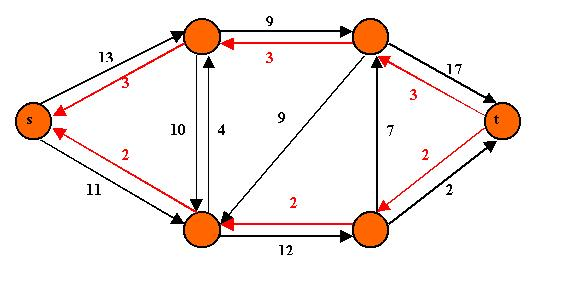
\includegraphics[width=0.5\textwidth]{./dados/figuras/figura1}
    \fonte{\citeonline{IRL2014}}
    \label{fig:figura-exemplo1}
\end{figure}

% QUADROS E TABELAS---------------------------------------------------------------
\chapter{QUADROS E TABELAS}
\label{chap:tabelas}

Exemplo de como inserir o \autoref{qua:quadro-exemplo1} e a \autoref{tab:tabela-exemplo1}. Ambos aparecem automaticamente nas suas respectivas listas. Para saber mais informações sobre a construção de tabelas no \LaTeX{} consulte literatura especializada \cite{Mittelbach2004}.

Ambos os elementos (Quadros e Tabelas) devem ser criados em arquivos separados para facilitar manutenção e armazenados no diretório de "/dados".

\begin{quadro}[!htb]
    \centering
    \caption{Exemplo de Quadro.\label{qua:quadro-exemplo1}}
    \begin{tabular}{|p{7cm}|p{7cm}|}
        \hline
        \textbf{BD Relacionais} & \textbf{BD Orientados a Objetos} \\
        \hline
        Os dados são passivos, ou seja, certas operações limitadas podem ser automaticamente acionadas quando os dados são usados. Os dados são ativos, ou seja, as solicitações fazem com que os objetos executem seus métodos. & Os processos que usam dados mudam constantemente. \\
        \hline
    \end{tabular}
    \fonte{\citeonline{Barbosa2004}}
\end{quadro}


A diferença entre quadro e tabela está no fato que um quadro é formado por linhas horizontais e verticais. Deve ser utilizado quando o conteúdo é majoritariamente não-numérico. O número do quadro e o título vem acima do quadro, e a fonte, deve vir abaixo. E Uma tabela é formada apenas por linhas verticais. Deve ser utilizada quando o conteúdo é majoritariamente numérico. O número da tabela e o título vem acima da tabela, e a fonte, deve vir abaixo, tal como no quadro.

\begin{table}[!htb]
    \centering
    \caption[Resultado dos testes]{Resultado dos testes.
    \label{tab:tabela-exemplo1}}
    \begin{tabular}{rrrrr}
        \toprule
            & Valores 1 & Valores 2 & Valores 3 & Valores 4 \\
        \midrule
            Caso 1 & 0,86 & 0,77 & 0,81 & 163 \\
            Caso 2 & 0,19 & 0,74 & 0,25 & 180 \\
            Caso 3 & 1,00 & 1,00 & 1,00 & 170 \\
        \bottomrule
    \end{tabular}
    \fonte{\citeonline{Barbosa2004}}
\end{table}


% EQUAÇÕES-----------------------------------------------------------------------
\chapter{EQUAÇÕES}
\label{chap:equacoes}

Exemplo de como inserir a \autoref{eq:equacao-exemplo1} e a Eq. \ref{eq:equacao-exemplo2} no corpo do texto \footnote{Deve-se atentar ao fato de a formatação das equações ficar muito boa esteticamente.}. Observe que foram utilizadas duas formas distintas para referenciar as equações.

\begin{equation}
    X(s) = \int\limits_{t = -\infty}^{\infty} x(t) \, \text{e}^{-st} \, dt
    \label{eq:equacao-exemplo1}
\end{equation}

\begin{equation}
    F(u, v) = \sum_{m = 0}^{M - 1} \sum_{n = 0}^{N - 1} f(m, n) \exp \left[ -j 2 \pi \left( \frac{u m}{M} + \frac{v n}{N} \right) \right]
    \label{eq:equacao-exemplo2}
\end{equation}

% ALGORITMOS-----------------------------------------------------------------------
\chapter{ALGORITMOS}
\label{chap:algoritmos}

Exemplo de como inserir um algoritmo. Para inserção de algoritmos utiliza-se o pacote {\ttfamily algorithm2e} que já está devidamente configurado dentro do template.

Os algoritmos devem ser criados em arquivos separados para facilitar manutenção e armazenados no diretório de "/dados".\\
\\

\begin{algorithm}
    \caption{Exemplo de Algoritmo}
    \KwIn{o número $n$ de vértices a remover, grafo original $G(V, E)$}
    \KwOut{grafo reduzido $G'(V,E)$}
    $removidos \leftarrow 0$ \\
    \While {removidos $<$ n } {
        $v \leftarrow$ Random$(1, ..., k) \in V$ \\
            \For {$u \in adjacentes(v)$} {
                remove aresta (u, v)\\
                $removidos \leftarrow removidos + 1$\\
            }
            \If {há  componentes desconectados} {
                remove os componentes desconectados\\
            }
        }
\end{algorithm}


% SOBRE AS LISTAS--------------------------------------------------------------------
\chapter{SOBRE AS LISTAS}
\label{chap:apSobreLista}

Para construir listas de "\textit{bullets}"{} ou listas enumeradas, inclusive listas aninhadas, é utilizado o pacote \verb|paralist|.

Exemplo de duas listas não numeradas aninhadas, utilizando o comando \verb|\itemize|. Observe a indentação, bem como a mudança automática do tipo de "\textit{bullet}"{} nas listas aninhadas.

\begin{itemize}
    \item item não numerado 1
    \item item não numerado 2
    \begin{itemize}
        \item subitem não numerado 1
        \item subitem não numerado 2
        \item subitem não numerado 3
    \end{itemize}
    \item item não numerado 3
\end{itemize}

Exemplo de duas listas numeradas aninhadas, utilizando o comando \verb|\enumerate|. Observe a numeração progressiva e indentação das listas aninhadas.

\begin{enumerate}
    \item item numerado 1
    \item item numerado 2
    \begin{enumerate}
        \item subitem numerado 1
        \item subitem numerado 2
        \item subitem numerado 3
    \end{enumerate}
    \item item numerado 3
\end{enumerate}

% SOBRE AS CITAÇÕES E CHAMADAS DE REFERÊNCAS----------------------------------------------
\chapter{SOBRE AS CITAÇÕES E CHAMADAS DE REFERÊNCAS}
\label{chap:apSobreCita}

Citações são trechos de texto ou informações obtidas de materiais consultadss quando da elaboração do trabalho. São utilizadas no texto com o propósito de esclarecer, completar e embasar as ideias do autor. Todas as publicações consultadas e utilizadas (por meio de citações) devem ser listadas, obrigatoriamente, nas referências bibliográficas, para preservar os direitos autorais. São classificadas em citações indiretas e diretas.

% CITAÇÕES INDIRETAS-----------------------------------------------------------------------
\chapter{CITAÇÕES INDIRETAS}
\label{chap:citacoesLivres}

É a transcrição, com suas próprias palavras, das idéias de um autor, mantendo-se o sentido original. A citação indireta é a maneira que o pesquisador tem de ler, compreender e gerar conhecimento a partir do conhecimento de outros autores. Quanto à chamada da referência, ela pode ser feita de duas maneiras distintas, conforme o nome do(s) autor(es) façam parte do seu texto ou não. Exemplo de chamada fazendo parte do texto:\\
\\Enquanto \citeonline{Maturana2003} defendem uma epistemologia baseada na biologia. Para os autores, é necessário rever \ldots.\\

A chamada de referência foi feita com o comando \verb|\citeonline{chave}|, que produzirá a formatação correta.

A segunda forma de fazer uma chamada de referência deve ser utilizada quando se quer evitar uma interrupção na sequência do texto, o que poderia, eventualmente, prejudicar a leitura. Assim, a citação é feita e imediatamente após a obra referenciada deve ser colocada entre parênteses. Porém, neste caso específico, o nome do autor deve vir em caixa alta, seguido do ano da publicação. Exemplo de chamada não fazendo parte do texto:\\
\\Há defensores da epistemologia baseada na biologia que argumentam em favor da necessidade de \ldots \cite{Maturana2003}.\\

Nesse caso a chamada de referência deve ser feita com o comando \verb|\cite{chave}|, que produzirá a formatação correta.

% CITAÇÕES DIRETAS-----------------------------------------------------------------------
\chapter{CITAÇÕES DIRETAS}
\label{chap:citacoesLiterais}

É a transcrição ou cópia de um parágrafo, de uma frase, de parte dela ou de uma expressão, usando exatamente as mesmas palavras adotadas pelo autor do trabalho consultado.

Quanto à chamada da referência, ela pode ser feita de qualquer das duas maneiras já mencionadas nas citações indiretas, conforme o nome do(s) autor(es) façam parte do texto ou não. Há duas maneiras distintas de se fazer uma citação direta, conforme o trecho citado seja longo ou curto.

Quando o trecho citado é longo (4 ou mais linhas) deve-se usar um parágrafo específico para a citação, na forma de um texto recuado (4 cm da margem esquerda), com tamanho de letra menor e espaçamento entrelinhas simples. Exemplo de citação longa:
\\\begin{citacao}
    Desse modo, opera-se uma ruptura decisiva entre a reflexividade filosófica, isto é a possibilidade do sujeito de pensar e de refletir, e a objetividade científica. Encontramo-nos num ponto em que o conhecimento científico está sem consciência. Sem consciência moral, sem consciência reflexiva e também subjetiva. Cada vez mais o desenvolvimento extraordinário do conhecimento científico vai tornar menos praticável a própria possibilidade de reflexão do sujeito sobre a sua pesquisa \cite[p.~28]{Silva2000}.
\end{citacao}

Para fazer a citação longa deve-se utilizar os seguintes comandos:
\begin{verbatim}
\begin{citacao}
<texto da citacao>
\end{citacao}
\end{verbatim}

No exemplo acima, para a chamada da referência o comando \verb|\cite[p.~28]{Silva2000}| foi utilizado, visto que os nomes dos autores não são parte do trecho citado. É necessário também indicar o número da página da obra citada que contém o trecho citado.

Quando o trecho citado é curto (3 ou menos linhas) ele deve inserido diretamente no texto entre aspas. Exemplos de citação curta:\\
\\A epistemologia baseada na biologia parte do princípio de que "assumo que não posso fazer referência a entidades independentes de mim para construir meu explicar" \cite[p.~35]{Maturana2003}.\\
\\A epistemologia baseada na biologia de \citeonline[p.~35]{Maturana2003} parte do princípio de que "assumo que não posso fazer referência a entidades independentes de mim para construir meu explicar".

% DETALHES SOBRE AS CHAMADAS DE REFERÊNCIAS---------------------------------------------------------
\chapter{DETALHES SOBRE AS CHAMADAS DE REFERÊNCIAS}
\label{chap:referUtilizadas}

Outros exemplos de comandos para as chamadas de referências e o resultado produzido por estes:\\
\\\citeonline{Maturana2003} \ \ \  \verb|\citeonline{Maturana2003}|\\
\citeonline{Barbosa2004} \ \ \   \verb|\citeonline{Barbosa2004}|\\
\cite[p.~28]{Silva2000} \ \ \  \verb|\cite[p.~28]{Silva2000}|\\
\citeonline[p.~33]{Silva2000} \ \ \   \verb|\citeonline[p.~33]{v}|\\
\cite[p.~35]{Maturana2003} \ \ \   \verb|\cite[p.~35]{Maturana2003}|\\
\citeonline[p.~35]{Maturana2003} \ \ \   \verb|\citeonline[p.~35]{Maturana2003}|\\
\cite{Barbosa2004,Maturana2003} \ \ \   \verb|\cite{Barbosa2004,Maturana2003}|\\

% SOBRE AS REFERÊNCIAS BIBLIOGRÁFICAS-------------------------------------------------------
\chapter{SOBRE AS REFERÊNCIAS BIBLIOGRÁFICAS}
\label{chap:apSobreRefer}

A bibliografia é feita no padrão \textsc{Bib}\TeX{}. As referências são colocadas em um arquivo separado. Neste template as referências são armazenadas no arquivo "base-referencias.bib".

Existem diversas categorias documentos e materiais componentes da bibliografia. A classe abn\TeX{} define as seguintes categorias (entradas):

\begin{verbatim}
@book
@inbook
@article
@phdthesis
@mastersthesis
@monography
@techreport
@manual
@proceedings
@inproceedings
@journalpart
@booklet
@patent
@unpublished
@misc
\end{verbatim}

Cada categoria (entrada) é formatada pelo pacote \citeonline{abnTeX22014d} de uma forma específica. Algumas entradas foram introduzidas especificamente para atender à norma \citeonline{NBR6023:2002}, são elas: \verb|@monography|, \verb|@journalpart|,\verb|@patent|. As demais entradas são padrão \textsc{Bib}\TeX{}. Para maiores detalhes, refira-se a \citeonline{abnTeX22014d}, \citeonline{abnTeX22014b}, \citeonline{abnTeX22014c}.

% NOTAS DE RODAPÉ--------------------------------------------------------------------------
\chapter{NOTAS DE RODAPÉ}
\label{chap:notasRodape}

As notas de rodapé pode ser classificadas em duas categorias: notas explicativas\footnote{é o tipo mais comum de notas que destacam, explicam e/ou complementam o que foi dito no corpo do texto, como esta nota de rodapé, por exemplo.} e notas de referências. A notas de referências, como o próprio nome ja indica, são utilizadas para colocar referências e/ou chamadas de referências sob certas condições.
                   % Capítulo com Orientações de uso do Template
% CONCLUSÃO--------------------------------------------------------------------

\chapter{CONCLUSÃO}
\label{chap:conclusao}

Parte final do texto, na qual se apresentam as conclusões do trabalho acadêmico. É importante fazer uma análise crítica do trabalho, destacando os principais resultados e as contribuições do trabalho para a área de pesquisa.

\section{TRABALHOS FUTUROS}
\label{sec:trabalhosFuturos}

Também deve indicar, se possível e/ou conveniente, como o trabalho pode ser estendido ou aprimorado.

\section{CONSIDERAÇÕES FINAIS}
\label{sec:consideracoesFinais}

Encerramento do trabalho acadêmico.
                 			   % Conclusão

\postextual
% INSERE ELEMENTOS PÓS-TEXTUAIS
% REFERÊNCIAS------------------------------------------------------------------

% Carrega o arquivo "base-referencias.bib" e extrai automaticamente as referências citadas

\bibliography{./base-referencias}
\bibliographystyle{abntex2-alf} % Define o estilo ABNT para formatar a lista de referências
% OBSERVAÇÕES------------------------------------------------------------------
% Este arquivo não precisa ser alterado.
           			   % Referências
% APÊNDICES--------------------------------------------------------------------

\begin{apendicesenv}
\partapendices

% Primeiro apêndice------------------------------------------------------------
\chapter{Nome do apêndice} % Edite para alterar o título deste apêndice
\label{chap:apendiceA}

Lembre-se que a diferença entre apêndice e anexo diz respeito à autoria do texto e/ou material ali colocado.

Caso o material ou texto suplementar ou complementar seja de sua autoria, então ele deverá ser colocado como um apêndice. Porém, caso a autoria seja de terceiros, então o material ou texto deverá ser colocado como anexo.

Caso seja conveniente, podem ser criados outros apêndices para o seu trabalho acadêmico. Basta recortar e colar este trecho neste mesmo documento. Lembre-se de alterar o "label"{} do apêndice.

Não é aconselhável colocar tudo que é complementar em um único apêndice. Organize os apêndices de modo que, em cada um deles, haja um único tipo de conteúdo. Isso facilita a leitura e compreensão para o leitor do trabalho.

% Novo apêndice----------------------------------------------------------------
\chapter{Nome do outro apêndice}
\label{chap:apendiceB}

conteúdo do novo apêndice

\end{apendicesenv}
             			   % Apêndices
% ANEXO------------------------------------------------------------------------

% \begin{anexosenv}
% \partanexos

% Primeiro anexo---------------------------------------------------------------
% \chapter{Nome do anexo}     % edite para alterar o título deste anexo
% \label{chap:anexoA}

% Lembre-se que a diferença entre apêndice e anexo diz respeito à autoria do texto e/ou material ali colocado.Caso o material ou texto suplementar ou complementar seja de sua autoria, então ele deverá ser colocado como um apêndice. Porém, caso a autoria seja de terceiros, então o material ou texto deverá ser colocado como anexo.Caso seja conveniente, podem ser criados outros anexos para o seu trabalho acadêmico. Basta recortar e colar este trecho neste mesmo documento. Lembre-se de alterar o "label"{} do anexo.Organize seus anexos de modo a que, em cada um deles, haja um único tipo de conteúdo. Isso facilita a leitura e compreensão para o leitor do trabalho. É para ele que você escreve.

% Novo anexo-------------------------------------------------------------------
% \chapter{Nome do outro anexo}
% \label{chap:anexoB}

% conteúdo do outro anexo

z% z\end{anexosenv}
               			   % Anexos

\end{document}
